\chapter{Lattice Gauge Theories}
\label{chap:intro}
In this chapter we will explore the theoretical framework we work within, essentially the fundamentals of Lattice Gauge Theories. Our understanding of Nature and its fundamental forces is best expressed through Quantum Field Theories (QFT), and in particular we will rely on the Path Integral formalism. The definition of Lattice Gauge Theories comes from the necessity to write the path integral of such theories in a completely non-perturbative fashion, hence we will see how to define their building blocks and how they tangle with computational physics, using the Schwinger Model as a reference.
\\ The Schwinger Model \cite{Schwinger:1962tp} consists of a two-dimensional realization of Quantum Electrodynamics (QED$_2$), hence a quantum field theory with U(1) gauge symmetry, embedded with two mass-degenerate dynamical quarks. This model has been the subject of many extensive studies throughout the last decades, as it shares interesting features with more realistic field theories, such as Quantum Chromodynamics (QCD). In the Schwinger Model one can observe quarks confinement, chiral symmetry breaking, the formation of a fermionic condensate and of a non-trivial topological $\theta-$vacuum \cite{COLEMAN1975267, COLEMAN1976239}, hence it can be used as a toy-model to test new computational methods, with cheaper computational costs.
\\ Before moving on to the case-study of this thesis, it is useful to recall some basic principles about Lattice Gauge Theories, in particular the definition of a U(1) Abelian Gauge theory on lattice and the implementation of dynamical fermions within it.

\section{QED: Continuum Formulation}
In this section we will briefly review how to derive the QED gauge-invariant action in the continuum formulation, before moving on to the lattice formulation. For a more complete description, it is convenient to check Quantum Field Theory books, such as \cite{Peskin:1995ev, Rothe:1992nt}.
\\ Quantum Electrodynamics can be described in terms of a quantum field theory characterized by a U(1) local symmetry, hence an abelian and continuous symmetry group. 
\\ The classic gauge-invariant action of the photon field $A_\mu(x)$ is given by:
\begin{equation}\label{S_G}
    S_G\,[A_\mu] = - \frac{1}{4} \int d^4x F_{\mu \nu}(x) F^{\mu\nu}(x)
\end{equation}
where $F_{\mu \nu} (x) = \partial_\mu A_\nu(x) - \partial_\nu A_\mu(x)$ is the gauge invariant field strength tensor, and $x \equiv x^\mu = (x^0, x^1, x^2, x^3)$ is a space-time point. The action $S_G$ is invariant under local transformations:
\begin{equation}
    A_\mu(x) \to A_\mu'(x) = A_\mu(x) + \partial_\mu g(x)
\end{equation}
where $g(x) = e^{i\Lambda(x)}$ is an element of the abelian U(1) group.
\\ Consider now the action of the free Dirac-field $\psi(x)$:
\begin{equation}
    S_F \, [\psi, \Bar{\psi}] = \int d^4 x \, \Bar{\psi}(x) \left(i \gamma^{\mu} \partial_\mu - m \right) \psi(x)
\end{equation}
where $\gamma_\mu$ are a set of $4 \times 4$ matrices which satisfy the Clifford algebra $\{\gamma^\mu, \gamma^\nu\} = 2 \eta^{\mu\nu}$, and $m$ is the mass parameter associated to the field $\psi$.
\\ The action $S_F$ is invariant under global U(1) transformations:
\begin{equation}\label{u(1) global}
    \begin{split}
        \psi (x) \to & \, \psi'(x) = e^{-iq\theta}\psi(x) \\
        \Bar{\psi} (x) \to & \, \Bar{\psi'}(x) = e^{iq\theta}\Bar{\psi}(x) \\
    \end{split}
\end{equation}
where $q$ is a label for the one-dimensional representations of the group, and coincides with the charge of the field $\psi$. For a collection of fields $\psi_i$, we could use independent transformations of the form (\ref{u(1) global}), leading to an action which is invariant under several copies of U(1). Nevertheless, we are interested in a common U(1) subgroup of these copies, such that each field $\psi_i$ transforms with the same group transformation $e^{iq_i\theta}$, but accordingly to different representations labelled by $q_i$.
\\ We now want to promote this global invariance of the Dirac equation to a local one, such that it coincides with the local U(1) invariance of the photon field. Consequently the QED action $S_{QED}$ will have a U(1) gauge symmetry, where fermions transform under unitary representations of U(1) labelled by their electric charge $q$. This can be achieved by means of the so called \textit{minimal transformation}, i.e. we replace the ordinary four-derivative $\partial_\mu$ with the covariant derivative $D_\mu$, defined by:
\begin{equation}
    D_\mu = \partial_\mu + iq A_\mu \hspace{10mm} \slashed{D} = i\gamma^\mu D_\mu
\end{equation}
which depends on the charge-representation it acts on. The resulting new action:
\begin{equation}\label{free Dirac cont}
    S_F \, [\psi, \Bar{\psi}] = \int d^4x \Bar{\psi}(x) (\slashed{D} - m) \psi(x)
\end{equation}
is invariant under the following set of local transformations:
\begin{equation}
\begin{split}
        \psi(x) & \to \psi'(x) = G(x) \psi(x) \\
    \Bar{\psi}(x) & \to \Bar{\psi'}(x) = \Bar{\psi}(x) G^{-1}(x) \\
    A_\mu (x) & \to A'_\mu(x) = G(x) A_\mu(x) G^{-1}(x) - \frac{i}{q} G(x) \partial_\mu G^{-1}(x) = A_\mu(x) - \frac{1}{q}\partial_\mu \Lambda(x)
\end{split}
\end{equation}
where
\begin{equation*}
    G(x) = e^{i\Lambda(x)} \in U(1).
\end{equation*}
The full gauge invariant action of QED is then given by:
\begin{equation}
    S_{QED} \, [A_\mu, \psi, \Bar{\psi}] = -\frac{1}{4}\int d^4x F^{\mu\nu}(x) F_{\mu\nu} + \int d^4x \Bar{\psi}(x) (\slashed{D} - m) \psi(x)
\end{equation}
Notice that the implementation of a local symmetry through the introduction of the covariant derivative naturally leads to the appearance of interacting terms in the action, i.e. the coupling between the EM field and the EM current $A_\mu (iq \Bar{\psi} \gamma^\mu \psi)$.
\\ The only way to define non-perturbatively a QFT consists in the implementation of the path-integral formalism, whose fundamental object is the partition function of the system. Before we build the QED partition function $Z_{QED}$, in order to define it rigorously we have to obtain the euclidean equivalent of the QED action. 
\\ Through the Wick rotation $(x^0 \to - ix_4)$ we switch to purely imaginary times, and consequently for the photon field we will substitute $(A^0 \to iA_4)$,\footnote{Since $(x^0 \to - ix_4)$ implies $(\partial_0 \to +i\partial_4)$, and $A_\mu$ could be a pure gauge configuration like $A_\mu = \partial_\mu \Lambda(x)$.} and the covariant derivative becomes $D_\mu = \partial_\mu + iqA_\mu$. Basically the euclidean action is given by $S^{E} = - i S$, where $S$ is simply the action in the Minkowski metric, so we obtain:
\begin{equation}
    S_{QED}^E \, [A_\mu, \psi, \Bar{\psi}]= \frac{1}{4} \int d^4 x F_{\mu\nu}(x) F_{\mu\nu}(x) + \int d^4x \Bar{\psi}(x) (\gamma_\mu D_\mu + m) \psi(x)
\end{equation}
where the sum over $\mu$ and $\nu$ is understood, and $\gamma_\mu$ (with $\mu = 1, \dots, 4$) are now the euclidean $\gamma$-matrices, which satisfy the relation $\{\gamma_\mu, \gamma_\nu\} = 2\delta_{\mu\nu}$. They are related to $\gamma$-matrices in the Minkowski space through the relations: $\gamma_4^E = \gamma^0, \gamma_i^E = -i\gamma^i$. 
\\ In order to achieve a completely non-perturbative definition of QED we need to take into consideration also the quantization-procedure of the photon field $A_\mu$ described by Faddeev and Popov \cite{FADDEEV196729}, which introduces a gauge-fixing term in the action, breaking explicitly the gauge-invariance of the action:
\begin{equation}\label{sqed}
    S = \frac{1}{4} \int d^4 x F_{\mu\nu}(x) F_{\mu\nu}(x) + \frac{1}{2\xi} \int d^4x (\partial_\mu A_\mu(x))^2 + \int d^4x \Bar{\psi}(x) (\gamma_\mu D_\mu + m) \psi(x)
\end{equation}
where $\xi$ is a gauge-fixing parameter. The partition function which defines QED non-perturbatively is then given by:
\begin{equation} 
    Z_{QED} = \int \prod_{\mu, x} A_\mu(x) \prod_{x, i, \alpha} \Bar{\psi}_{i,\alpha}(x) \prod_{x, i, \alpha} \psi_{i, \alpha}(x) \, e^{-S} = \int \mathcal{D}A_\mu \mathcal{D}\Bar{\psi} \mathcal{D}\psi \, e^{-S}
\end{equation}
where $i$ is an index which labels the fermionic flavors we are taking into account, while $\alpha$ labels the fermionic degrees of freedom.
\\ This is a formal expression which should be managed with care, especially for what concerns the integration measure, whose equivalent will be clear in the lattice formulation.
\\ Unfortunately, the only non-perturbative definition of QED in the continuum formulation is the trivial one, where the coupling constant is identically null.
\\ Now we want to move towards a definition of QED in the lattice formulation, and our first ingredient will be the implementation of fermions on a four-dimensional space-time lattice. 

\newpage

\section{Fermions on lattice}
In this section we will explore one of the required ingredients to define a quantum field theory on lattice, matter fields or \textit{fermions}. \\ Fermions obey, as their name suggests, a Fermi-Dirac statistics, hence they are antisymmetric under the exchange of any pair of quantum numbers. This kind of statistics can be embedded by the so-called \textit{Grassmann variables} for quark fields, i.e. anti-commuting numbers. If we were to discretize fermions naively, we would have to face the appearance of some unphysical lattice artifacts, the so-called \textit{doublers}. After we investigate the nature of these objects, culminating in the enunciate of the Nielsen-Ninomiya theorem \cite{NIELSEN198120}, we will show how to remove the doublers by adding an extra term to the fermion action, leading to the so-called \textit{Wilson fermion action.}

\subsection{Naive discretization of free fermions}
As a first step in the definition of the lattice formulation, we introduce a four-dimensional hypercube $\Lambda$ of lattice spacing $a$ to resemble our space-time. Each point $n$ of the lattice is labelled by four integers $n = (n_1, n_2, n_3, n_4)$, and if we call $N_1 = N_2 = N_3 = N$ the spatial extent in each direction, and $N_0$ the time extent of the lattice, we will have:
\begin{equation}\label{lattice}
\begin{split}
        \Lambda = \{ n = (n_1, n_2, n_3, n_4 \} | 
        \,\, 0 \leq n_{1,2,3} \leq N - 1, \,\,\,
        0 \leq n_4 \leq N_0 - 1 \}
\end{split}
\end{equation}
and we will typically refer to the integer-valued coordinate $n$ of each reticular site, rather then its actual space-time position $x = an.$
\\ At each lattice site we define a pair of spinorial fields $\psi_{\alpha, f}(n)$ and $\Bar{\psi}_{\alpha', f'}(n)$, and each field carries Dirac ($\alpha, \alpha'$) and flavor indices ($f, f'$), as they did in the continuum. Since all fermionic degrees of freedom in our theory must anti-commute with each other, their path integral must be built using adequate variables that resemble this property. This can be achieved by means of the so-called Grassmann variables, hence anti-commuting numbers, which allow us to reinforce the following relations for a set of fermionic fields\footnote{If we were to consider strong interactions as well, we would add a third quantum number $a$, associated with the color charge of the fermion field.}:
\begin{equation}
    \begin{split}
        \psi_{\alpha, f}(n) \psi_{\alpha', f'}(n') = - \psi_{\alpha', f'}'(n') \psi_{\alpha, f}(n) \\
        \Bar{\psi}_{\alpha, f}(n) \Bar{\psi}_{\alpha', f'}(n') = - \Bar{\psi}_{\alpha', f'}'(n') \Bar{\psi}_{\alpha, f}(n) \\
        \psi_{\alpha, f}(n) \Bar{\psi}_{\alpha', f'}(n') = - \Bar{\psi}_{\alpha', f'}'(n') \psi_{\alpha, f}(n) 
    \end{split}
\end{equation}
Grassmann variables follow some non-trivial algebra relations, whose consequences are crucial for the study of fermions in lattice gauge theories. We won't report all the details of Grassmann algebras, which can be found in standard textbooks like \cite{Rothe:1992nt, Gattringer:2010zz}.
\\ Recall the expression for the free Dirac action in the continuum euclidean formulation:
\begin{equation}\label{S_f cont}
    S_F \, [\psi, \Bar{\psi}] = \int d^4x \Bar{\psi}(x) (\gamma_\mu \partial_\mu + m) \psi(x)
\end{equation}
the most naive way to write a possible lattice equivalent comes from the discretization of this integral, where we substitute the partial derivative with an equivalent discrete expression. If we define the \textit{forward} and \textit{backward derivative} respectively as:
\begin{equation}
    D_\mu \psi(n) = \frac{\psi(n + \hat{\mu}) - \psi(n)}{a} \hspace{10mm} D^*_\mu \psi(n) = \frac{\psi(n) - \psi(n - \hat{\mu})}{a}
\end{equation}
where $\hat{\mu}$ is a unit vector in the direction $\mu$, we can build the \textit{symmetric derivative}:
\begin{equation}
    \partial_\mu \psi(x) \to \frac{1}{2} \left( D_\mu + D_\mu^*\right)\psi(n) = \frac{1}{2a}\left(\psi(n + \hat{\mu}) - \psi(n - \hat{\mu}) \right)
\end{equation}
which is affected by $\mathcal{O}(a^2)$ discretization errors, compared to the $\mathcal{O}(a)$ errors of the forward and backward derivatives. By plugging this definition in (\ref{S_f cont}), we get a naive version of the lattice fermionic action:
\begin{equation}
    S_F\,[\psi, \Bar{\psi}] = a^4 \sum_{n \in \Lambda} \frac{1}{2a}\left[ \Bar{\psi}(n) \gamma_\mu \psi(n + \hat{\mu}) - \Bar{\psi}(n) \gamma_\mu \psi(n - \hat{\mu})  \right] + m \Bar{\psi}(n) \psi(n)
\end{equation}
which can be rewritten in a quadratic form as:
\begin{equation}\label{S naive}
     S_F\,[\psi, \Bar{\psi}] = a^4 \sum_{n, m \in \Lambda} \sum_{\alpha, \beta} \Bar{\psi}_{\alpha}(n) K_{\alpha, \beta}(n, m) \psi_\beta(m)
\end{equation}
if we define:
\begin{equation}\label{K}
    K_{\alpha, \beta}(n, m) = \sum_{\mu = 1}^4 \left( \gamma_\mu \right)_{\alpha, \beta} \frac{\delta_{n + \hat{\mu}, m} - \delta_{n - \hat{\mu},m} }{2a}
\end{equation}
Up to now we stressed repetitively the word \textit{naive}, and indeed this comes from the fact that this action is not a good discretization of the free-Dirac field action on lattice. \\ To see this, it is convenient to study $S_F$ in momentum space, hence we need to define the Fourier Transform on lattice (see \cite{Gattringer:2010zz} for more details). We defined our lattice $\Lambda$ in (\ref{lattice}), and $\abs{\Lambda}$ will refer to the hypervolume of our hypercube, hence $\abs{\Lambda} = N^3 N_0$. We want to impose toroidal boundary condition, which can be expressed as:
\begin{equation}
    f(n + \hat{\mu}n_\mu) = e^{i2\pi \theta_\mu} f(n) \hspace{10mm} \forall \mu
\end{equation}
Here $n_\mu$ simply denotes four sets of integers, one for each direction $\mu$, while $\theta_\mu$ is a parameter which allows us to express more compactly periodic and anti-periodic boundary conditions, since $\theta_\mu = 0$ for directions where PBC hold, and $\theta_\mu = \frac{1}{2}$ for directions with APBC. From the formalization of our momentum space $\Tilde{\Lambda}$:
\begin{equation}
    \Tilde{\Lambda} = \biggl\{ p = (p_1, p_2, p_3, p_4) \, | \, p_\mu = \frac{2\pi}{a n_\mu}(k_\mu + \theta_\mu); k_\mu = - \frac{n_\mu}{2} + 1, \dots, \frac{n_\mu}{2} \biggr\}
\end{equation}
it follows that $p_\mu$ can range in $\left(-\frac{\pi}{a}, \frac{\pi}{a} \right]$, and we can identify the boundaries of this Brillouin Zone (BZ). It is easy to show that in this framework, we can introduce two useful relations:
\begin{equation}
    \frac{1}{\abs{\Lambda}} \sum_{p \in \Tilde{\Lambda}} \exp(ip \cdot (n - n')a) = \delta(n - n') = \delta_{n_1, n_1'}\delta_{n_2, n_2'}\delta_{n_3, n_3'}\delta_{n_4, n_4'}
\end{equation}
\begin{equation}
    \frac{1}{\abs{\Lambda}} \sum_{n \in \Lambda} \exp(i(p - p') \cdot na) = \delta(p - p') = \delta_{k_1, k_1'}\delta_{k_2, k_2'}\delta_{k_3, k_3'}\delta_{k_4, k_4'}
\end{equation}
where $p \cdot (n - n') \equiv p_\mu (n_\mu - n_\mu')$, and $k_\mu$ label the components of $p_\mu$.
\\ The definition of the Fourier Transform of a function $f(n)$ is then given by:
\begin{equation}
    \Tilde{f}(p) = \frac{1}{\sqrt{\abs{\Lambda}}} \sum_{n \in \Lambda} f(n) \exp(-ip\cdot n a)
\end{equation}
and the inverse Fourier Transform is:
\begin{equation}
    f(n) = \frac{1}{\sqrt{\abs{\Lambda}}} \sum_{p \in \Tilde{\Lambda}} \Tilde{f}(p) \exp(i p \cdot na)
\end{equation}
If we apply the FT to the kernel of the free Dirac action $K(n, m)$, we obtain:
\begin{equation}
    \begin{split}
        \Tilde{K}(p, q) & = \frac{1}{\abs{\Lambda}}\sum_{n, m} e^{-ip\cdot na} K(n,m) e^{iq \cdot na} = \\
                        & = \frac{1}{\abs{\Lambda}}\sum_{n, m} e^{-i(p-q)\cdot na} \left( \sum_{\mu = 1}^4 \gamma_\mu \frac{e^{iq_\mu a} - e^{-i q_\mu a}}{2a} + m\mathbb{1} \right) \\
                        & = \delta(p - q) \left[ m \mathbb{1} + \frac{i}{a} \gamma_\mu \sin(p_\mu a) \right] = \delta(p - q) \Tilde{K}(p)
    \end{split}
\end{equation}
where the sum over $\mu$ is understood in the last line. Notice that the discretization of the momentum:
\begin{equation}
    \Bar{p}_\mu = \frac{1}{a} \sin(p_\mu a)
\end{equation}
correctly tends to $p_\mu$ if we take the naive continuum limit $a \to 0$. 
\\ It is easy to show that the fermion-propagator $\Tilde{K}^{-1}(p)$ is given by:
\begin{equation}
    \Tilde{K}^{-1}(p) = \frac{m\mathbb{1} - i \gamma_\mu \Bar{p_\mu}}{m^2 + \sum_\mu \Bar{p}_\mu^2}
\end{equation}
and one could confidently say that, in the massless fermion limit ($m = 0$), it has the correct naive continuum limit:
\begin{equation}
    \Tilde{K}^{-1}(p) \bigg\rvert_{m = 0} = \frac{-i \gamma_\mu \Bar{p}_\mu}{\sum_\mu \Bar{p}_\mu}^2 \xrightarrow[\Bar{p}_\mu \to p_\mu]{\mathit{a \to 0}} \frac{-i \gamma_\mu p_\mu}{\sum_\mu p_\mu^2}
\end{equation}
But here comes the problem: we cannot substitute $\Bar{p}_\mu$ with $p_\mu$ in the propagator. Indeed, $\Bar{p}_\mu$ vanishes for $p_\mu = 0, \pm \frac{\pi}{a}$, hence the discretized momentum is zero also at the boundaries of the Brillouin Zone over which we integrate!
This leads to unphysical poles in the propagator $\Bar{K}^{-1}(p)$ at:
\begin{equation}
    p = \left(\frac{\pi}{a}, 0, 0, 0\right), \left(0, \frac{\pi}{a}, 0, 0 \right), \dots, \left(\frac{\pi}{a}, \frac{\pi}{a}, \frac{\pi}{a}, \frac{\pi}{a}\right)
\end{equation}
while the pole at $p = \left(0, 0, 0, 0 \right)$ is the only physical one. Altogether, we get 16 poles in the propagator for a four-dimensional space-time lattice, the so-called \textit{doublers} (there would have been $2^D$ doublers in $D$ dimensions), hence the naive discretization of the Dirac equation describes the kinematics of 16 mass-degenerate fermionic particles.
\\ \begin{figure}[H]
    \centering
    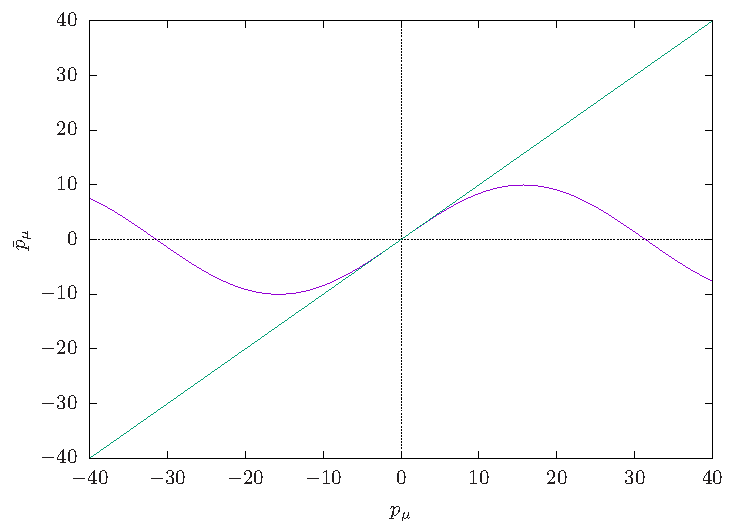
\includegraphics[width = 8 cm]{images/pbar.pdf}
    \caption{Violet curve: $\Bar{p}_\mu = \frac{1}{a} \sin(p_\mu a)$, $a = 0.1$. Green curve: $\Bar{p}_\mu = p_\mu$}
    \label{fig: pbar vs p}
\end{figure} 
Figure (\ref{fig: pbar vs p}) shows how for large momenta, where $p_\mu$ and $\Bar{p}_\mu$ are of the order of $a^{-1}$, the deviation from the $\Bar{p}_\mu = p_\mu$ line is not negligible, and we have high momentum excitations also for $a \to 0$.
The propagator, which in the space regime coincides with the fermionic two-point function, takes contributions from 16 fermion-like particles, which are pure lattice artifacts with no continuum analog.
\\ The origin of doublers has a precise meaning, since it is tangled with the chiral anomaly of our theory.
In the massless fermion limit ($m = 0$), the continuum QED action (\ref{sqed}) is invariant under the global chiral transformation:
\begin{equation}
    \psi \to e^{i\theta \gamma_5} \psi \hspace{15mm} \Bar{\psi} \to \Bar{\psi} e^{i\theta \gamma_5}
\end{equation}
where $\theta$ is a parameter and $\gamma_5 = \gamma_1 \gamma_2 \gamma_3 \gamma_4$ is an hermitian matrix which anticommutes with any $\gamma_\mu$. Since for any global symmetry we expect a conserved current, the global chiral symmetry implies the existence of a conserved axial-vector current, but due to quantum fluctuation it diverges anomalously in the continuum theory. When we regularize the theory on lattice and try to preserve chiral symmetry, we implicitly impose that this current is strictly conserved for any $a$, hence the lattice finds a way to cancel the anomaly of the continuum limit, associated with momentum excitations around $p = 0.$
\\ The appearence of doublers must occur in a lattice regularization which respects $\gamma_5$-hermiticity, locality and translational invariance, as it is formalized in the Nielsen-Ninomiya No Go Theorem \cite{NIELSEN198120}. The theorem states that, given a lattice regularization of the Dirac equation, its kernel $\Tilde{K}(p)$ in momentum space cannot satisfy the following conditions simultaneously:
\begin{enumerate}
    \item $\Tilde{K}(p)$ is a smooth function of momenta $p_\mu$, with period $\frac{2\pi}{a}$.
    \item In the massless fermions limit, $\Tilde{K}(p)$ reduces to the continuum Dirac operator for $a \to 0$.
    \item $\Tilde{K}(p)$ is invertible $\forall p \neq 0.$
    \item In the massless fermions limit, $\Tilde{K}(p)$ satisfies: $\{\Tilde{K}(p), \gamma_5 \} = 0.$
\end{enumerate}
Hence the action (\ref{S naive}) lead to the appearance of doublers because it implicitly required invariance under chiral symmetry! As a consequence, in order to remove these unphysical objects, one needs to sacrifice chiral symmetry. 

\subsection{Wilson fermion}
In this framework, a possible solution was proposed by Wilson. The idea consists in a modification of the Dirac action, such that in the naive continuum limit $a \to 0$ it reduces to the standard formulation and takes care of doublers. As we mentioned before, the price to pay is the breaking of chiral symmetry, which is puzzling but does not spoil the definition of our theory on lattice, as it is a global symmetry of QED rather than a defining one. 
\\ Wilson proposed the following Dirac-operator:
\begin{equation}
    D^{(W)} = \frac{1}{2} \{ \gamma_\mu (D_\mu^* + D_\mu) - r D_\mu^\dagger D_\mu \}
\end{equation}
where $r$ is the so-called Wilson parameter (we will fix $r = 1$ in our case study). This expression differs from the naive discretization of the Dirac operator because of the second term, which is a gauge-invariant discrete version of the euclidean D'Alambertian $\Box$. \\ The Wilson-modified action is then given by:
\begin{equation}
    S_F^{(W)} = a^4 \sum_{n, m \in \Lambda} \Bar{\psi}_\alpha(n) K_{\alpha, \beta}^{(W)}(n, m) \psi_\beta(m)
\end{equation}
with:
\begin{equation}
\begin{split}
        K_{\alpha, \beta}^{(W)}(n, m) & = D^{(W)}_{\alpha, \beta}(n,m) - m \delta_{\alpha, \beta}\delta_{m,n} \\
         & = (m + 2r)\delta_{\alpha, \beta}\delta_{m,n} - \frac{1}{2}\sum_\mu \left[(r - \gamma_\mu)_{\alpha, \beta} \delta_{m, n+\hat{\mu}} + (r + \gamma_\mu)_{\alpha, \beta} \delta_{m, n - \hat{\mu}} \right]
\end{split}
\end{equation}
Notice that for $r \neq 0$, this definition breaks chiral symmetry even for $m \to 0$.
\\ One can prove that the kernel in momentum space $\Tilde{K}^{(W)}(p)$ does not satisfy the anticommuting condition with $\gamma_5$, hence it can obey all the remaining conditions of the Nielsen-Ninomiya theorem. 
In particular, the Dirac-Wilson operator takes care of doublers, because the $\mathcal{O}(a)$ term introduced by Wilson changes the propagator and gives to the unphysical excitations a mass proportional to $a^{-1}$, which diverges for $a \to 0$. 
\\ Indeed, one can show that:
\begin{equation}
    \Tilde{K}_W (p) = i \gamma_\mu \Bar{p}_\mu + m\mathbb{1} + \frac{a}{2} \hat{p}^2 \hspace{4mm} \mbox{with} \hspace{4 mm} \hat{p}_\mu = \frac{2}{a} \sin(\frac{p_\mu a}{2})
\end{equation}
and from an analysis similar to the naive case, the propagator is now given by (in the massless fermions limit $m = 0$):
\begin{equation}
    \frac{-i \gamma_\mu \Bar{p}_\mu + \frac{a}{2} \hat{p}^2}{\sum_\mu \Bar{p}_\mu^2 + (\frac{a}{2} \hat{p}^2)^2}
\end{equation}
In the directions associated with doublers ($p_\mu = \pm \pi/a$), we get $\hat{p}_\mu = \pm 2/a$, hence the mass associated to the unphysical excitation is proportional to $\frac{1}{a} \xrightarrow{a \to 0} \infty$, so that these degrees of freedom decouple from our theory in the continuum limit. The pole in $p = 0$ is the only one with vanishing mass for $a \to 0$, hence Wilson's proposal is a good discretization of the continuum Dirac action.
\\ It is good to remark that there are other working solution in literature, such as \textit{staggered fermions}, but in our work we will deal with Wilson fermions.

\section{Compact QED: Lattice Formulation}
We can finally conclude the construction of the lattice QED action. This process will follow two basic requirements, i.e. the action should be locally invariant under $U(1)$ transformations and should reduce to the classical continuum action in the naive continuum limit.
\\ The QED action should contain a fermion part and a gauge part, just like in the continuum formulation, and we should start with the fermionic term. Recall the lattice action for a free Dirac field:
\begin{equation}
\begin{split}
    & S_F^{(W)} [\psi, \Bar{\psi}] = (m + 2r)\sum_{n \in \Lambda} \Bar{\psi}(n)\psi(n) - \\ & \hspace{20mm} - \frac{1}{2}\sum_{n, \mu} \left[\Bar{\psi}(n)(r - \gamma_\mu)_{\alpha, \beta} \psi(n + \hat{\mu}) + \Bar{\psi}(n + \hat{\mu})(r + \gamma_\mu)_{\alpha, \beta} \psi(n) \right]
\end{split}
\end{equation}
This expression is invariant under the global U(1) transformation:
\begin{equation*}
    \begin{split}
       & \psi(n) \to G\psi(n) \\
       & \Bar{\psi}(n) \to \Bar{\psi}(n) G^{-1}
    \end{split}
\end{equation*}
where $G \in U(1).$ We want to promote this global symmetry to a local one, hence in the previous relations the group element should depend on the lattice site $G(n).$ \\ This could seem to be problematic, as the fermion action includes terms which are non-diagonal in the lattice site, e.g. $\Bar{\psi}(n)\gamma_\mu\psi(n + \hat{\mu})$. Anyway, the puzzle can easily be solved thanks to an idea developed, again, by Wilson: we will introduce new degrees of freedom, which will embed the gauge fields contribution in our theory in a gauge-invariant fashion and will allow us to implement a local $U(1)$ gauge invariance.
\\ Let's see how the problem would be handled in the continuum. Given a bilinear $\Bar{\psi}(x) \psi(y)$, generally it is not invariant under a local gauge transformation:
\begin{equation*}
    \Bar{\psi}(x) \psi(y) \to \Bar{\psi}^G(x) \psi^G(y) = \Bar{\psi}(x) G^{-1}(x) G(y) \psi(y) \Rightarrow G^{-1} (x) G(y) \neq \mathbb{1}
\end{equation*}
In order to make it gauge-invariant, we must compensate the variation $G^\dagger (x) G(y)$ by introducing a factor which depends on the gauge potential, the so called \textit{Schwinger line integral}:
\begin{equation}
    U(x, y) = e^{i\int_x^y dz_\mu A_\mu(z)}
\end{equation}
where $z_\mu$ is a unit vector tangent to the path $C$ connecting $x$ and $y$ (the sum over $\mu$ is understood). One can prove easily that under a gauge transformation $A_\mu \to A_\mu - \frac{1}{e} \partial_\mu A_\mu$, the Schwinger line transforms covariantly:
\begin{equation}\label{bil1}
    U(x, y) \to U^G(x,y) = G(x) U(x, y) G^{-1}(y)
\end{equation}
hence we can build a gauge-invariant object as $\Bar{\psi}(x) U(x, y) \psi(y)$. If we fix $y = x + \varepsilon$ and take $\varepsilon \to 0$, we can expand the previous contraction, and with a little algebra one gets to the result:
\begin{equation}\label{bil2}
    \Bar{\psi}(x) U(x, x + \varepsilon) \psi(x + \varepsilon) = \Bar{\psi}(x) \psi(x) + \varepsilon \Bar{\psi}(x) \left( \partial_\mu + i e A_\mu \right) \psi(x) + \mathcal{O}(\varepsilon^2)
\end{equation}
From this expression, we read that the Schwinger line is essentially a generalization of the covariant derivative when $x$ and $y$ are not at an infinitesimal distance. Since on a lattice our fields are necessarily defined at a finite distance, Wilson conjectured that one could use Schwinger lines as the fundamental degrees of freedom of lattice gauge theories, instead of the gauge fields we used to build the covariant derivative. This will lead to a modification of the gauge action, which is nevertheless legitimate: any regularization on lattice suffers from discretization errors which cancel out in the continuum limit, so one can modify these errors in order to preserve an exact gauge invariance for the action of our theory.
\\ Notice that we are substituting gauge fields, objects which live in the algebra of the gauge group, with Schwinger lines between two adjacent point of the lattice, hence elements of the gauge group. As Schwinger lines connect different points of the lattice, we will also call them \textit{links}. For instance, the discrete form of our gauge field will be given by a $U(1)$ element, which can be written as:
\begin{equation}
    U_\mu (n) = e^{i \phi_\mu (n)}
\end{equation}
where $\phi_\mu$ is a real-valued variable which takes values in $[0, 2\pi]$, and this objects lives on the link connecting the lattice site $n$ to an adjacent one $n + \hat{\mu}$, with $\mu = \{0, 1, 2, 3\}$. One can prove that, in order to have the correct naive continuum limit for the QED action, we can establish a relation between the phase $\phi_\mu(n)$ and the vector potential $A_\mu(n)$, so that we should actually consider the identification\footnote{Note that the identification of $A_\mu(n)$ with the vector potential is strictly true only in the continuum limit.}:
\begin{equation}
    U_\mu (n) = e^{iea A_\mu(n)}
\end{equation}
\begin{center}



\tikzset{every picture/.style={line width=0.75pt}} %set default line width to 0.75pt        

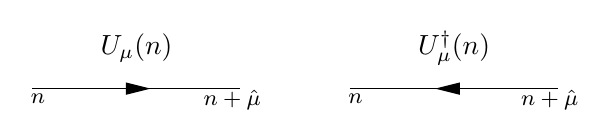
\begin{tikzpicture}[x=0.75pt,y=0.75pt,yscale=-1,xscale=1]
%uncomment if require: \path (0,82); %set diagram left start at 0, and has height of 82

%Straight Lines [id:da540606925296075] 
\draw    (198,40.71) -- (298,40.71) ;
\draw [shift={(255,40.71)}, rotate = 180] [fill={rgb, 255:red, 0; green, 0; blue, 0 }  ][line width=0.08]  [draw opacity=0] (12,-3) -- (0,0) -- (12,3) -- cycle    ;
%Straight Lines [id:da6698465419967881] 
\draw    (351,40.71) -- (451,40.71) ;
\draw [shift={(392,40.71)}, rotate = 0] [fill={rgb, 255:red, 0; green, 0; blue, 0 }  ][line width=0.08]  [draw opacity=0] (12,-3) -- (0,0) -- (12,3) -- cycle    ;


% Text Node
\draw (196,42.11) node [anchor=north west][inner sep=0.75pt]  [font=\footnotesize]  {${\textstyle n}$};
% Text Node
\draw (279.2,40.11) node [anchor=north west][inner sep=0.75pt]  [font=\footnotesize]  {${\textstyle n+\hat{\mu }}$};
% Text Node
\draw (229.6,13.11) node [anchor=north west][inner sep=0.75pt]    {$U_{\mu }( n)$};
% Text Node
\draw (349,42.11) node [anchor=north west][inner sep=0.75pt]  [font=\footnotesize]  {${\textstyle n}$};
% Text Node
\draw (432.2,40.11) node [anchor=north west][inner sep=0.75pt]  [font=\footnotesize]  {${\textstyle n+\hat{\mu }}$};
% Text Node
\draw (382.6,11.61) node [anchor=north west][inner sep=0.75pt]    {$U_{\mu }^{\dagger }( n)$};


\end{tikzpicture}
\end{center}
\\ As we can see in the drawing above, links are directed quantities, so the complex conjugate will be defined as:
\begin{equation}\label{U}
    U_\mu^\dagger(n) = e^{-ieaA_\mu(n)}
\end{equation}
and will connect the lattice site $n + \hat{\mu}$ to $n$. In analogy to what we have described in the continuum formulation in (\ref{bil1})-(\ref{bil2}), the non-diagonal terms of the fermionic action will become:
\begin{equation}
    \begin{split}
        & \Bar{\psi}(n) (r - \gamma_\mu) \psi(n + \hat{\mu}) \to \Bar{\psi}(n) (r - \gamma_\mu) U_\mu(n) \psi(n + \hat{\mu}) \\
        & \Bar{\psi}(n + \hat{\mu}) (r + \gamma_\mu) \psi(n) \to \Bar{\psi}(n + \hat{\mu}) (r + \gamma_\mu) U_\mu^\dagger(n) \psi(n)
    \end{split}
\end{equation}
and these expressions are now invariant under the set of local transformations:
\begin{equation}
    \begin{split}
        & \psi(n) \to G(n) \psi(n) \hspace{33 mm} \Bar{\psi}(n) \to \Bar{\psi}(n) G^{-1} (n) \\
        & U_\mu(n) \to G(n) U_\mu(n) G^{-1}(n + \hat{\mu}) \hspace{10 mm} U_\mu^\dagger(n) \to G(n + \hat{\mu}) U_\mu^\dagger(n) G^{-1}(n)
    \end{split}
\end{equation}
By requiring such transformation laws, we can implement the $U(1)$ gauge invariance naturally. The idea that links should be group elements, rather than elements of the group algebra, comes from the fact that also their gauge transforms must be $U(1)$ elements.
\\ Finally, we can write the gauge invariant action for Wilson fermions on lattice:
\begin{equation}
    \begin{split}
        & S_F^{(W)} [\psi, \Bar{\psi}, U] = (m + 2r) \sum_{n \in \Lambda} \Bar{\psi}(n) \psi(n) - \\
        & \hspace{25 mm} - \frac{1}{2} \sum_{n, \mu} \left[ \Bar{\psi}(n) (r - \gamma_\mu) U_\mu(n) \psi(n + \hat{\mu}) + \Bar{\psi}(n + \hat{\mu}) (r + \gamma_\mu) U_\mu^\dagger(n) \psi(n) \right]
    \end{split}
\end{equation}
and by replacing $U_\mu(n) \simeq 1 + i e a A_\mu(n)$ for small values of $a$, one can show that $S_F^{(W)}$ reduces to the continuum expression in the naive continuum limit.
\\ In order to complete our lattice description of QED, we should now take care of the gauge-invariant discretization of the gauge action, embedding the link variables we just introduced. It turns out that the easiest local object that allows us to build a gauge-invariant realization is the so-called \textit{plaquette}, i.e. the smallest counterclockwise path-ordered product of link variables, as shown below:
\begin{equation}
    U_{\mu\nu}(n) = U_\mu(n) U_\nu(n + \hat{\mu}) U_\mu^\dagger(n + \hat{\nu}) U_\nu^\dagger(n)
\end{equation}
\begin{center}
    
\tikzset{every picture/.style={line width=0.75pt}} %set default line width to 0.75pt        

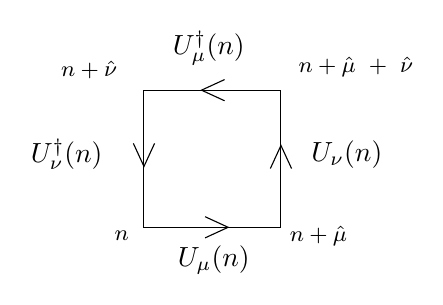
\begin{tikzpicture}[x=0.75pt,y=0.75pt,yscale=-1,xscale=1]
%uncomment if require: \path (0,182); %set diagram left start at 0, and has height of 182

%Shape: Square [id:dp08152467645896022] 
\draw   (297.13,62.23) -- (363.15,62.23) -- (363.15,128.25) -- (297.13,128.25) -- cycle ;
\draw   (326.6,123.23) -- (337.72,128.34) -- (326.6,133.45) ;
\draw   (336,57.17) -- (324.88,62.27) -- (336,67.38) ;
\draw   (302.27,87.92) -- (297.16,99.03) -- (292.05,87.92) ;
\draw   (358.05,100.03) -- (363.16,88.92) -- (368.27,100.03) ;


% Text Node
\draw (281.8,128.91) node [anchor=north west][inner sep=0.75pt]  [font=\footnotesize]  {${\textstyle n}$};
% Text Node
\draw (366.2,126.31) node [anchor=north west][inner sep=0.75pt]  [font=\footnotesize]  {${\textstyle n+\hat{\mu }}$};
% Text Node
\draw (312.2,136.11) node [anchor=north west][inner sep=0.75pt]    {$U_{\mu }( n)$};
% Text Node
\draw (370.4,45.23) node [anchor=north west][inner sep=0.75pt]  [font=\footnotesize]  {${\textstyle n+\hat{\mu } \ +\ \hat{\nu }}$};
% Text Node
\draw (256,47.23) node [anchor=north west][inner sep=0.75pt]  [font=\footnotesize]  {${\textstyle n+\hat{\nu }}$};
% Text Node
\draw (376.6,85.23) node [anchor=north west][inner sep=0.75pt]    {$U_{\nu }( n)$};
% Text Node
\draw (309.8,32.43) node [anchor=north west][inner sep=0.75pt]    {$U_{\mu }^{\dagger }( n)$};
% Text Node
\draw (241.4,84.43) node [anchor=north west][inner sep=0.75pt]    {$U_{\nu }^{\dagger }( n)$};

\end{tikzpicture}
\end{center}
Using the expression for $U_\mu(n)$ (\ref{U}), one can show that the plaquette reduces to:
\begin{equation}
    U_{\mu\nu}(n) = e^{iea^2F_{\mu\nu}(n)}
\end{equation}
where $F_{\mu\nu}$ is a discretization of the continuum electromagnetic field strength tensor:
\begin{equation}
    F_{\mu\nu}(n) = \frac{1}{a}\left[(A_\nu(n + \hat{\mu}) - A_\nu(n)) - (A_\mu(n + \hat{\nu}) - A_\mu(n)) \right]
\end{equation}
In order to reproduce the continuum action (\ref{S_G}), we need to take a particular combination:
\begin{equation}
    \frac{1}{e^2} \sum_n \sum_{\substack{\mu, \nu \\ \mu < \nu}} \left[1 - \frac{1}{2} \left(U_{\mu\nu}(n) + U_{\mu\nu}^\dagger(n)\right) \right] \approx \frac{1}{4} \sum_{\substack{n \\ \mu, \nu}} a^4 F_{\mu\nu}(n) F_{\mu\nu}(n)
\end{equation}
which can be recast more compactly as:
\begin{equation}
    S_G [U] = \frac{\beta}{2} \sum_P \left[1 - \Re{U_P} \right]
\end{equation}
with $\beta = 2/e^2$, and the sum over $P$ labels a summation over all the plaquettes of the lattice. Comparing this expression with the continuum formulation of QED, one can notice that the coupling constant now appears as $1/e$ in the gauge action, rather than with a linear dependence in the fermionic part. This suggests that the strong coupling expansion is the most natural one in the lattice formulation of the theory.
\\ Now we can write the lattice action for QED with Wilson fermions, which will be at the base of our path-integral formalism:
\begin{equation}\label{S qed lattice}
    \begin{split}
       & S_{QED} [\psi, \Bar{\psi}, U] = S_G[U] + S_F^{(W)} [\psi, \Bar{\psi}] = \\
       & \hspace{23 mm} = \frac{\beta}{2} \sum_P \left[1 - \Re{U_P} \right] + (m + 2r) \sum_{n \in \Lambda} \Bar{\psi}(n) \psi(n) - \\
       & \hspace{36 mm} - \frac{1}{2} \sum_{n, \mu} \left[ \Bar{\psi}(n) (r - \gamma_\mu) U_\mu(n) \psi(n + \hat{\mu}) + \Bar{\psi}(n + \hat{\mu}) (r + \gamma_\mu) U_\mu^\dagger(n) \psi(n) \right] \\
    \end{split}
\end{equation}
The QED partition function will involve an integration over all possible fermionic and gauge fields configurations. The fermionic measure is given by the integration over two sets of Grassmann variables $[\psi, \Bar{\psi}]$, while the link variables $U_\mu(n)$ are elements of the unitary group $U(1)$, so we are integrating over a compact group manifold, which in this case is parameterised by a single real-valued variable $\phi_\mu(n)$ restricted to the range $[0, 2\pi]$. \\ Then we can build the gauge-invariant measure:
\begin{equation}
    \mathcal{D}U \equiv \prod_{n, \mu} d\phi_\mu(n)
\end{equation}
and the QED partition function is given by:
\begin{equation}
    Z_{QED} = \int \mathcal{D}U \mathcal{D}\psi \mathcal{D}\Bar{\psi} \, e^{-S_{QED}[\psi, \Bar{\psi}, U]}
\end{equation}
As a final remark, when we build an interacting theory from this partition function, we shall remember that the parameters $m$ and $e$ that appear in (\ref{S qed lattice}) cannot be interpreted as the physical fermion mass and electric charge, but should rather be regarded as bare parameters with no direct physical meaning.
\\ This completes the review of the theoretical framework of this thesis, so now we can focus more in detail on the case study of our work, the Schwinger Model.